\documentclass[gray]{beamer}
\usepackage[utf8]{inputenc}
\usepackage[T2A]{fontenc}
\usepackage[english,russian]{babel}
\usepackage{newtxtext,newtxmath}
\usepackage{graphicx} % Пакет для работы с изображениями
\usepackage{adjustbox} % Hyperlinks
\usepackage{courier}
\usepackage{blindtext}

\usepackage{float}
\usepackage{listings}

\definecolor{c}{HTML}{000050}

\usetheme{default}

\setbeamertemplate{footline}[frame number]
\setbeamertemplate{navigation symbols}{}

\begin{document}

\begingroup
\setbeamertemplate{footline}{}
\begin{frame}
%\begin{center}
    % \hfill
    \begin{minipage}{0.1\textwidth}
        
\includegraphics[width=1.7cm]{img/bmstu.pdf}
    \end{minipage}
    % \hspace{1cm}
    \hfill
    \begin{minipage}{0.8\textwidth}\centering\bfseries
        {
            \linespread{1}\selectfont\tiny
            \vspace{0.1cm}
            {Министерство~науки~и~высшего~образования~Российской~Федерации}

            {Федеральное~государственное~бюджетное~образовательное~учреждение высшего~образования}

            {
                <<Московский~государственный~технический~университет

                имени~Н.Э.~Баумана

                (национальный~исследовательский~университет)>>
            }

            {(МГТУ им. Н.Э.~Баумана)}
            \vspace{0.1cm}
        }
    \end{minipage}

    \vspace{0.2cm}
    %\rule{\linewidth}{2.8pt}
    \rule[3ex]{\linewidth}{1pt}

    \vfill

    \begin{center}
    \Large Методы выделения составных частей научного текста
    \end{center}

    \vfill

    \begin{minipage}[t]{0.45\textwidth}
        \small
        \raggedright
        Выполнил:

        студент 4 курса

        группы ИУ7-74Б

        \makebox[0pt][l]{Рунов Константин Алексеевич}
    \end{minipage}
    \hfill
    \begin{minipage}[t]{0.45\textwidth}
        \small
        \raggedleft
        Руководитель:

        \makebox[0pt][r]{Строганов Юрий Владимирович}
    \end{minipage}

    \vfill

    \begin{center}
        Москва, \the\year\ г.
    \end{center}
\end{frame}
\endgroup

\begin{frame}
    \frametitle{Цель и задачи}
    Целью данной работы является классификация методов выделения составных частей научного текста.

    \vfill

    Задачи:
    \begin{itemize}
        \item провести анализ предметных областей анализа структуры документов и научно-технических текстов;
        \item провести обзор существующих методов выделения составных частей научного текста;
        \item сформулировать критерии сравнения описанных методов;
        \item провести классификацию описанных методов по сформулированным критериям.
    \end{itemize}
\end{frame}

\begin{frame}
    \frametitle{Анализ предметной области. Анализ структуры документов}
    \centering
    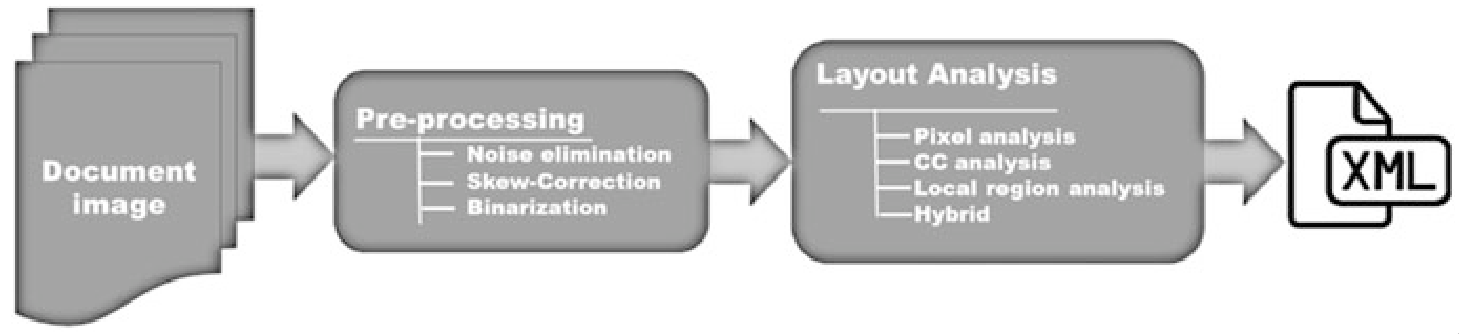
\includegraphics[width=\textwidth]{img/typical-dla-system.png}
\end{frame}

\begin{frame}
    \frametitle{Анализ предметной области. Типы макетов документов}
    \centering
    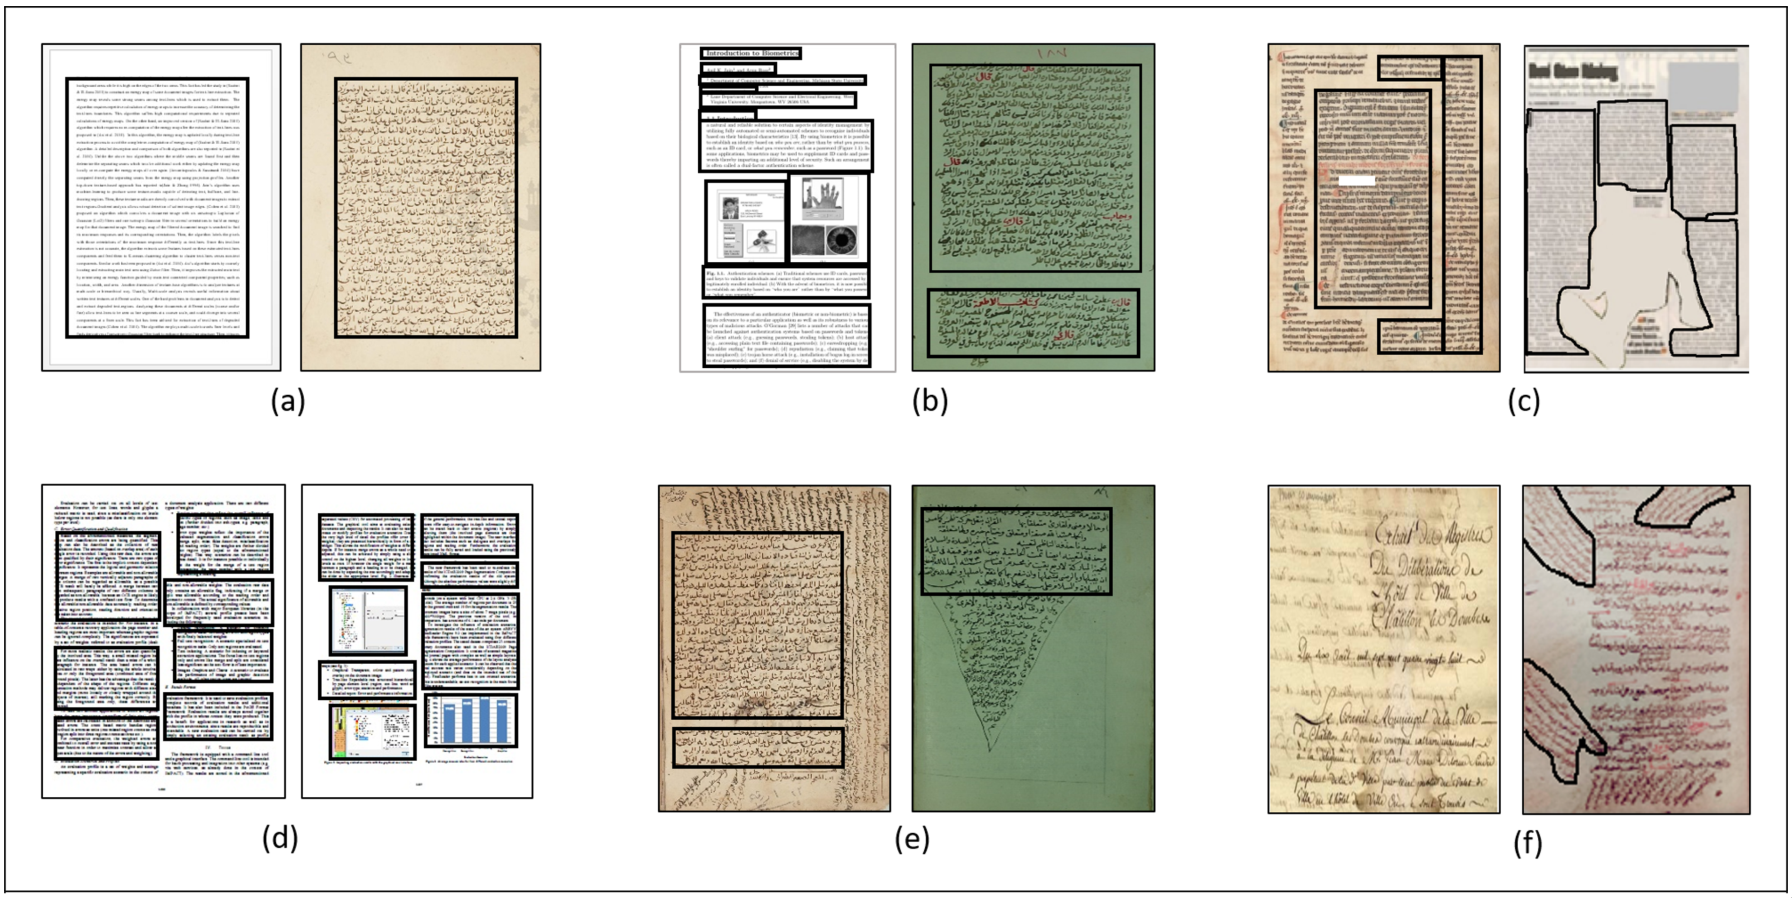
\includegraphics[width=\textwidth]{img/layouts.png}
\end{frame}

\begin{frame}
    \frametitle{Анализ предметной области. Структура научного текста}
    \centering
    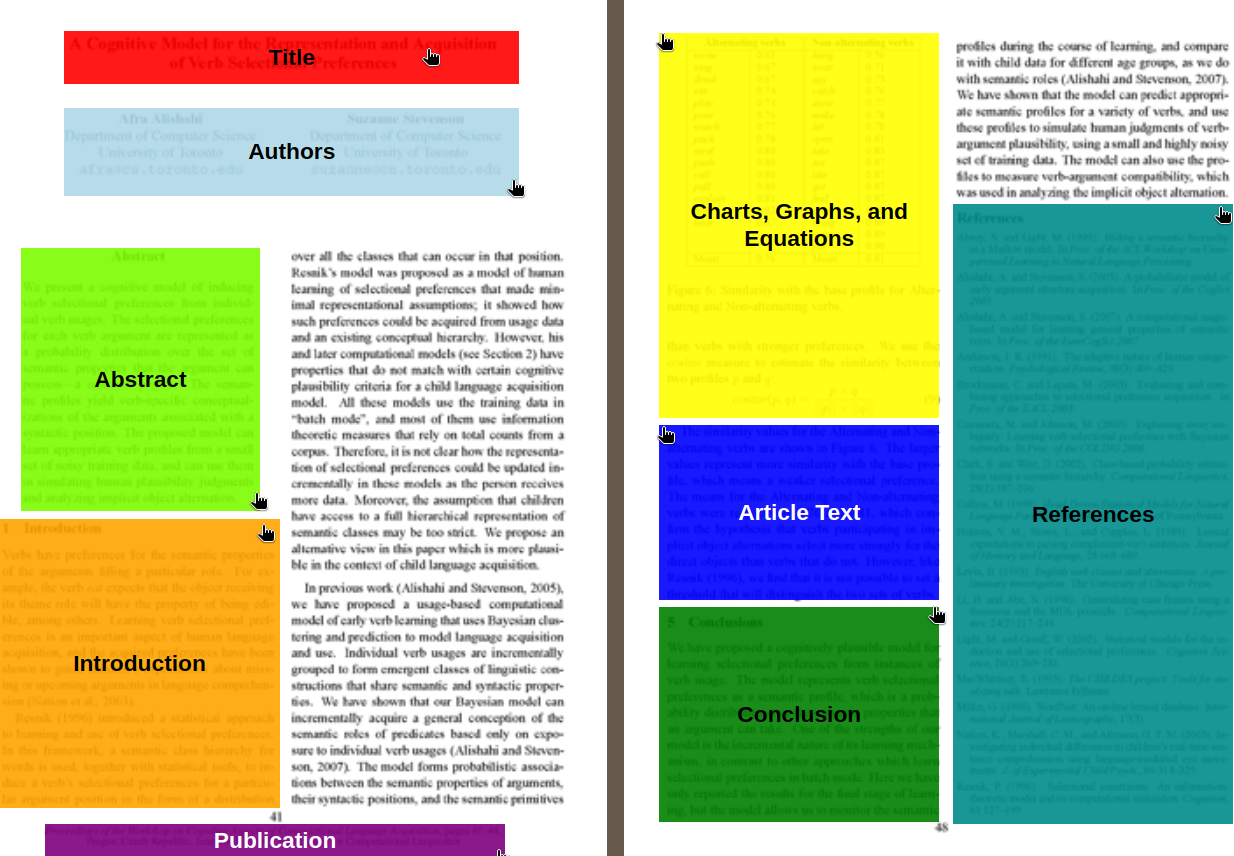
\includegraphics[width=\textwidth]{img/struct-parts-named.png}
\end{frame}

\begin{frame}
    \frametitle{Классификация методов}
    \centering

    \begin{table}[H]
        \centering
        \caption{Классификация методов DLA}
        \label{tab:table}
    \resizebox{\linewidth}{!}{% Resize table to fit within \linewidth horizontally
        \begin{tabular}{|c|c|c|c|c|}
            \hline
            \textbf{Метод} & \textbf{Стратегия} & \textbf{Скорость} & \textbf{Гибкость} & \textbf{Устойчивость} \\ \hline
            CCA        & Снизу вверх & 2 & 2 & 3 \\ \hline
            PPA        & Сверху вниз & 2 & 3 & 3 \\ \hline
            RLSA       & Сверху вниз & 1 & 3 & 3 \\ \hline
            ML         & Снизу вверх & 3 & 1 & 1 \\ \hline
            PPA + CCA  & Гибридный   & 2 & 3 & 2 \\ \hline
        \end{tabular}
        }
    \end{table}
\end{frame}

\begin{frame}
    \frametitle{Заключение}
Цель данной работы, а именно классификация методов выделения составных частей научного текста, была достигнута.

Для достижения поставленной цели были решены следующие задачи:
\begin{itemize}
    \item проведен анализ предметных областей анализа структуры документов и научно-технических текстов;
    \item проведен обзор существующих методов выделения составных частей научного текста;
    \item сформулированы критерии сравнения описанных методов;
    \item проведена классификация описанных методов по сформулированным критериям.
\end{itemize}
\end{frame}

\end{document}
